\documentclass{standalone}

\usepackage{tikz}
\usepackage{standalone}
\usetikzlibrary{calc}
\usepackage{color}

\usetikzlibrary{decorations.pathmorphing}
\usetikzlibrary{fit}					% fitting shapes to coordinates
\usetikzlibrary{backgrounds}	% drawing the background after the foreground

\tikzstyle{background}=[red, rectangle, draw, inner sep=0.1mm,
		   rounded corners=3mm]

\begin{document}

    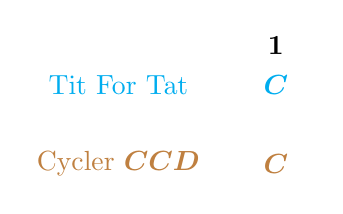
\begin{tikzpicture}

    \tikzstyle{state}=[minimum width=1cm, font=\boldmath];
    

	\node[thick] (0) at (-1, 0) [state] {\textcolor{cyan}{Tit For Tat}};
	\node[thick] (1) at (-1, -1) [state] {\textcolor{brown}{Cycler $CCD$}};

	\node[thick] (2) at (1, 0.5) [state] {$1$};

	\node (8) at (1, 0) [state] {\textcolor{cyan}{$C$}};

	\node (14) at (1, -1) [state] {\textcolor{brown}{$C$}};

    \end{tikzpicture}

\end{document}